% coding:utf-8

%FOSAET, a LaTeX-Code for a electrical summary of basic electronics
%Copyright (C) 2013, Daniel Winz, Ervin Mazlagic

%This program is free software; you can redistribute it and/or
%modify it under the terms of the GNU General Public License
%as published by the Free Software Foundation; either version 2
%of the License, or (at your option) any later version.

%This program is distributed in the hope that it will be useful,
%but WITHOUT ANY WARRANTY; without even the implied warranty of
%MERCHANTABILITY or FITNESS FOR A PARTICULAR PURPOSE.  See the
%GNU General Public License for more details.
%----------------------------------------

\chapter{Formelsammlung}
\newpage
% \begin{figure}[h!]
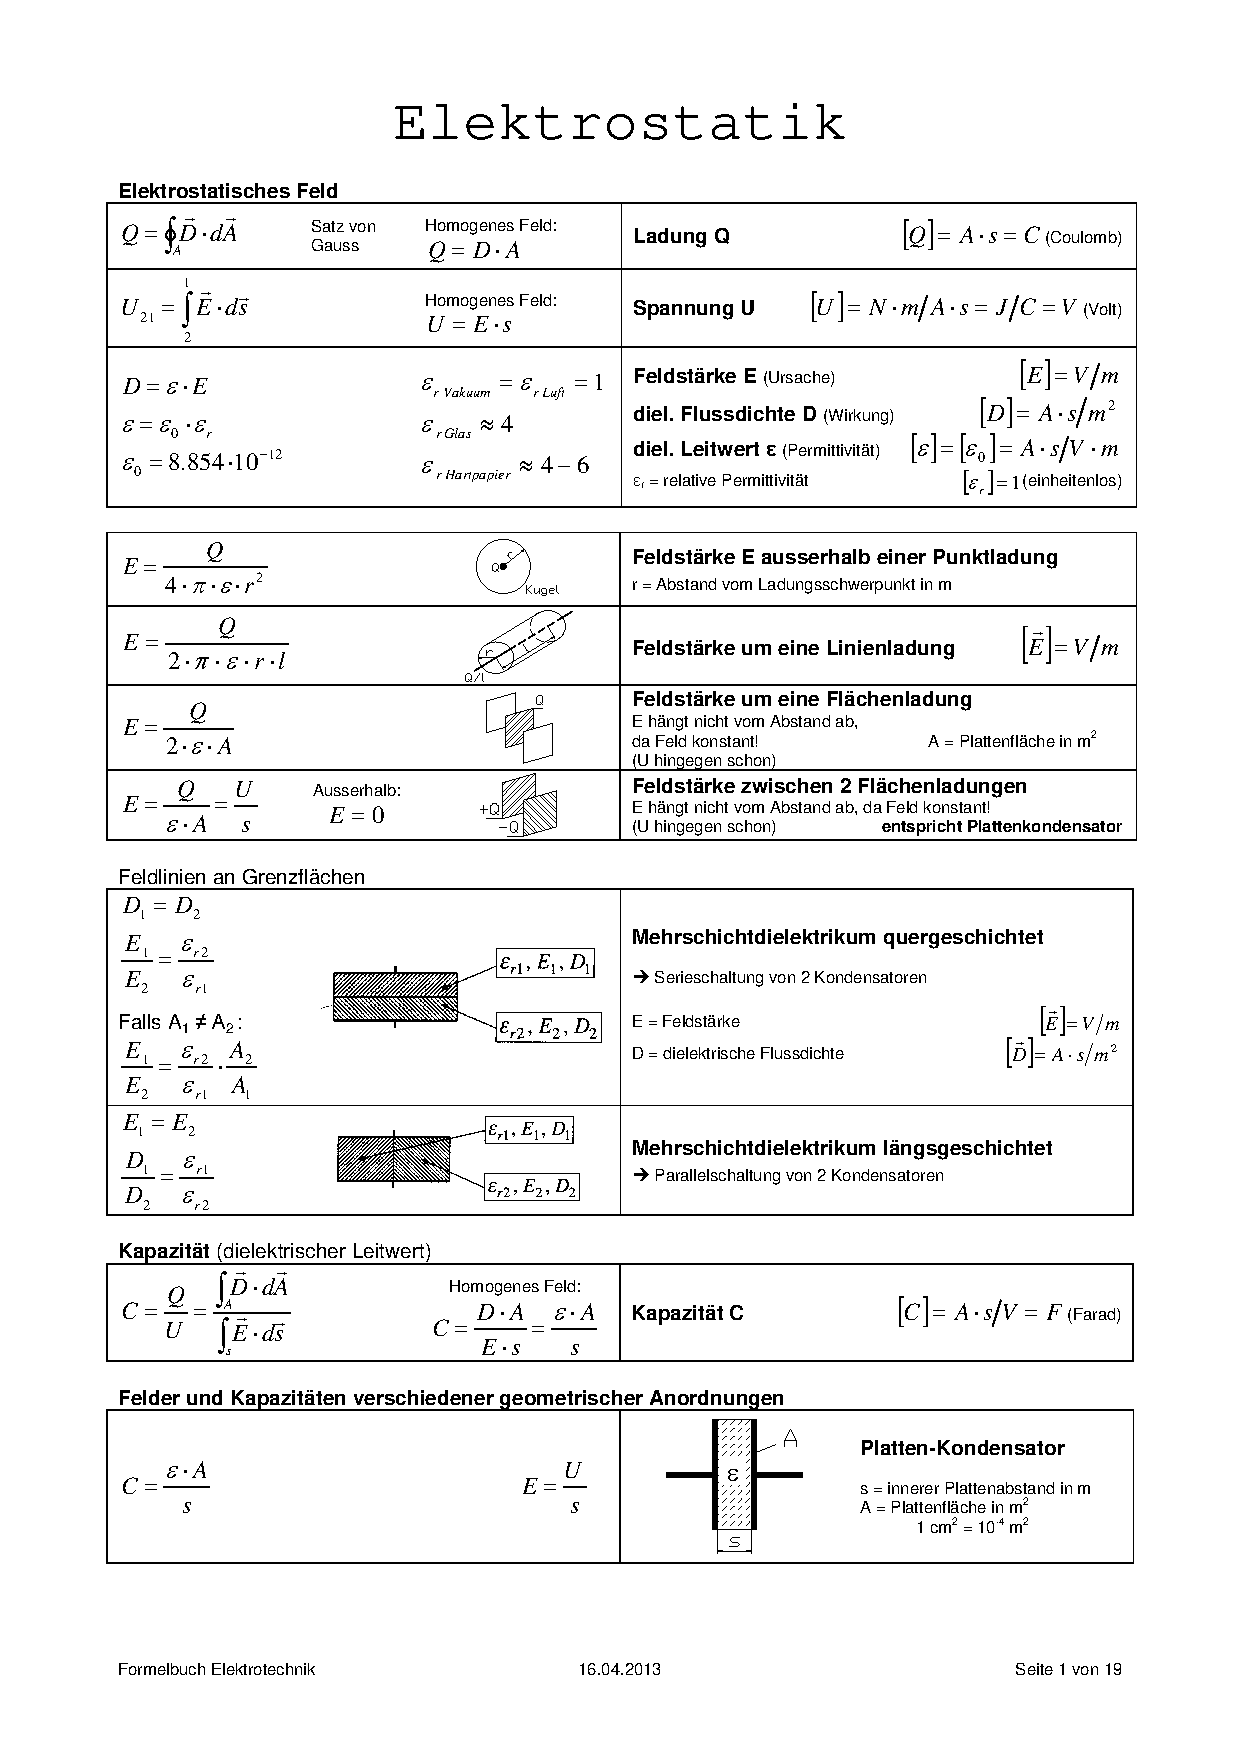
\includegraphics[page=1,scale=0.57,trim=20mm 20mm 20mm 20mm]{ET-Formelsammlung}
% \end{figure}
\newpage
% \begin{figure}[h!]
\includegraphics[page=2,scale=0.57,trim=20mm 20mm 20mm 20mm]{ET-Formelsammlung}
% \end{figure}
\newpage
% \begin{figure}[h!]
\includegraphics[page=3,scale=0.57,trim=20mm 20mm 20mm 20mm]{ET-Formelsammlung}
% \end{figure}
\newpage
% \begin{figure}[h!]
\includegraphics[page=4,scale=0.57,trim=20mm 20mm 20mm 20mm]{ET-Formelsammlung}
% \end{figure}
\newpage
% \begin{figure}[h!]
\includegraphics[page=5,scale=0.57,trim=20mm 20mm 20mm 20mm]{ET-Formelsammlung}
% \end{figure}
\newpage
% \begin{figure}[h!]
\includegraphics[page=6,scale=0.57,trim=20mm 20mm 20mm 20mm]{ET-Formelsammlung}
% \end{figure}
\newpage
% \begin{figure}[h!]
\includegraphics[page=7,scale=0.57,trim=20mm 20mm 20mm 20mm]{ET-Formelsammlung}
% \end{figure}
\newpage
% \begin{figure}[h!]
\includegraphics[page=8,scale=0.57,trim=20mm 20mm 20mm 20mm]{ET-Formelsammlung}
% \end{figure}
\newpage
% \begin{figure}[h!]
\includegraphics[page=9,scale=0.57,trim=20mm 20mm 20mm 20mm]{ET-Formelsammlung}
% \end{figure}
\newpage
% \begin{figure}[h!]
\includegraphics[page=10,scale=0.57,trim=20mm 20mm 20mm 20mm]{ET-Formelsammlung}
% \end{figure}
\newpage
% \begin{figure}[h!]
\includegraphics[page=11,scale=0.57,trim=20mm 20mm 20mm 20mm]{ET-Formelsammlung}
% \end{figure}
\newpage
% \begin{figure}[h!]
\includegraphics[page=12,scale=0.57,trim=20mm 20mm 20mm 20mm]{ET-Formelsammlung}
% \end{figure}
\newpage
% \begin{figure}[h!]
\includegraphics[page=13,scale=0.57,trim=20mm 20mm 20mm 20mm]{ET-Formelsammlung}
% \end{figure}
\newpage
% \begin{figure}[h!]
\includegraphics[page=14,scale=0.57,trim=20mm 20mm 20mm 20mm]{ET-Formelsammlung}
% \end{figure}
\newpage
% \begin{figure}[h!]
\includegraphics[page=15,scale=0.57,trim=20mm 20mm 20mm 20mm]{ET-Formelsammlung}
% \end{figure}
\newpage
% \begin{figure}[h!]
\includegraphics[page=16,scale=0.57,trim=20mm 20mm 20mm 20mm]{ET-Formelsammlung}
% \end{figure}
\newpage
% \begin{figure}[h!]
\includegraphics[page=17,scale=0.57,trim=20mm 20mm 20mm 20mm]{ET-Formelsammlung}
% \end{figure}
\newpage
% \begin{figure}[h!]
\includegraphics[page=18,scale=0.57,trim=20mm 20mm 20mm 20mm]{ET-Formelsammlung}
% \end{figure}
\newpage
% \begin{figure}[h!]
\includegraphics[page=19,scale=0.57,trim=20mm 20mm 20mm 20mm]{ET-Formelsammlung}
% \end{figure}
\\
\\
Quelle: Ilias ET2